\documentclass[11pt,t]{beamer}
\usetheme{Malmoe}
\usepackage[utf8]{inputenc}
\usepackage{amsmath}
\usepackage{amsfonts}
\usepackage{amssymb}
\usepackage[all,cmtip]{xy}
\usepackage{pgfpages}
\usepackage{graphicx}

\pgfpagesuselayout{resize to}[letterpaper,landscape,border shrink=5mm]
\newenvironment{amatrix}[1]{%
  \left[\begin{array}{@{}*{#1}{c}|c@{}}
}{%
  \end{array}\right]
}
\DeclareMathOperator{\rank}{rank}
\DeclareMathOperator{\minor}{minor}
\DeclareMathOperator{\cof}{cof}
\DeclareMathOperator{\adj}{adj}
\DeclareMathOperator{\spn}{span}

\newcommand{\R}{\mathbb{R}}
\newcommand{\C}{\mathbb{C}}
\renewcommand{\Re}{\operatorname{Re}}
\renewcommand{\Im}{\operatorname{Im}}
\newcommand{\abs}[1]{\lvert #1\rvert}
\newcommand{\len}[1]{\lVert #1\rVert}
\newcommand{\dotp}{\boldsymbol{\cdot}}
\newcommand{\comp}[2]{\operatorname{comp}_{\vec{#1}}\vec{#2}}
\newcommand{\proj}[2]{\operatorname{proj}_{\vec{#1}}\vec{#2}}
%\geometry{landscape,paper=letterpaper}
\beamertemplatenavigationsymbolsempty
\date{}
\author{Math 1410 Linear Algebra}
\title{Complex Numbers}
%\setbeamercovered{transparent} 
%\setbeamertemplate{navigation symbols}{} 
%\logo{} 
%\institute{} 
%\date{} 
%\subject{} 
\begin{document}
\begin{frame}
\titlepage
\end{frame}

%\begin{frame}
%\tableofcontents
%\end{frame}

\begin{frame}\frametitle{The complex number system}
We define the set of \alert{complex numbers}, denoted $\C$, as
\[
 \C = \{x+iy\,|\, x,y\in\R\},
\]
where $i$ denotes a (non-real) number with the property that $i^2=-1$.

\begin{itemize}
 \item Complex numbers date back to 16th-century Italy, and Cardano's {\em Ars Magna} (1545).
 \item Used (relucantly) by Bombelli to solve equations in 1572.
 \item Largely ignored as nonsense for 250 years. (Some dabbling by Euler around 1770.)
 \item Acceptance follows geometric interpretation by Gauss, Argand, and others at the end of the 18th century.
 \item Most development of the subject (by Cauchy, Riemann, et al) took place between 1814 and 1851.
\end{itemize} 
\end{frame}
\begin{frame}\frametitle{Bombelli and the cubic}
\begin{itemize}
 \item Many texts (incorrectly) assert that complex numbers arose out of the need to solve quadratic equations like $x^2+1=0$.
 \item This is historically false: geometrically no solutions were expected.
 \item First compelling reason was the \alert{cubic} equation $x^3=3px+2q$.
 \item Cubic formula due to Cardano:
\[
 x = \sqrt[3]{q+\sqrt{q^2-p^3}}+\sqrt[3]{q-\sqrt{q^2-p^3}}
\]
 \item Result is a real number even if there are negative numbers under the square roots.
\end{itemize}

\end{frame}
\begin{frame}\frametitle{The Argand Plane}
 Geometrically, we identify $z=x+iy\in \C$ with $(x,y)\in\R^2$. This visualization is usually called the \alert{Argand plane} or \alert{Gauss plane}, after the mathematicians who introducded this point of view.
\begin{center}
 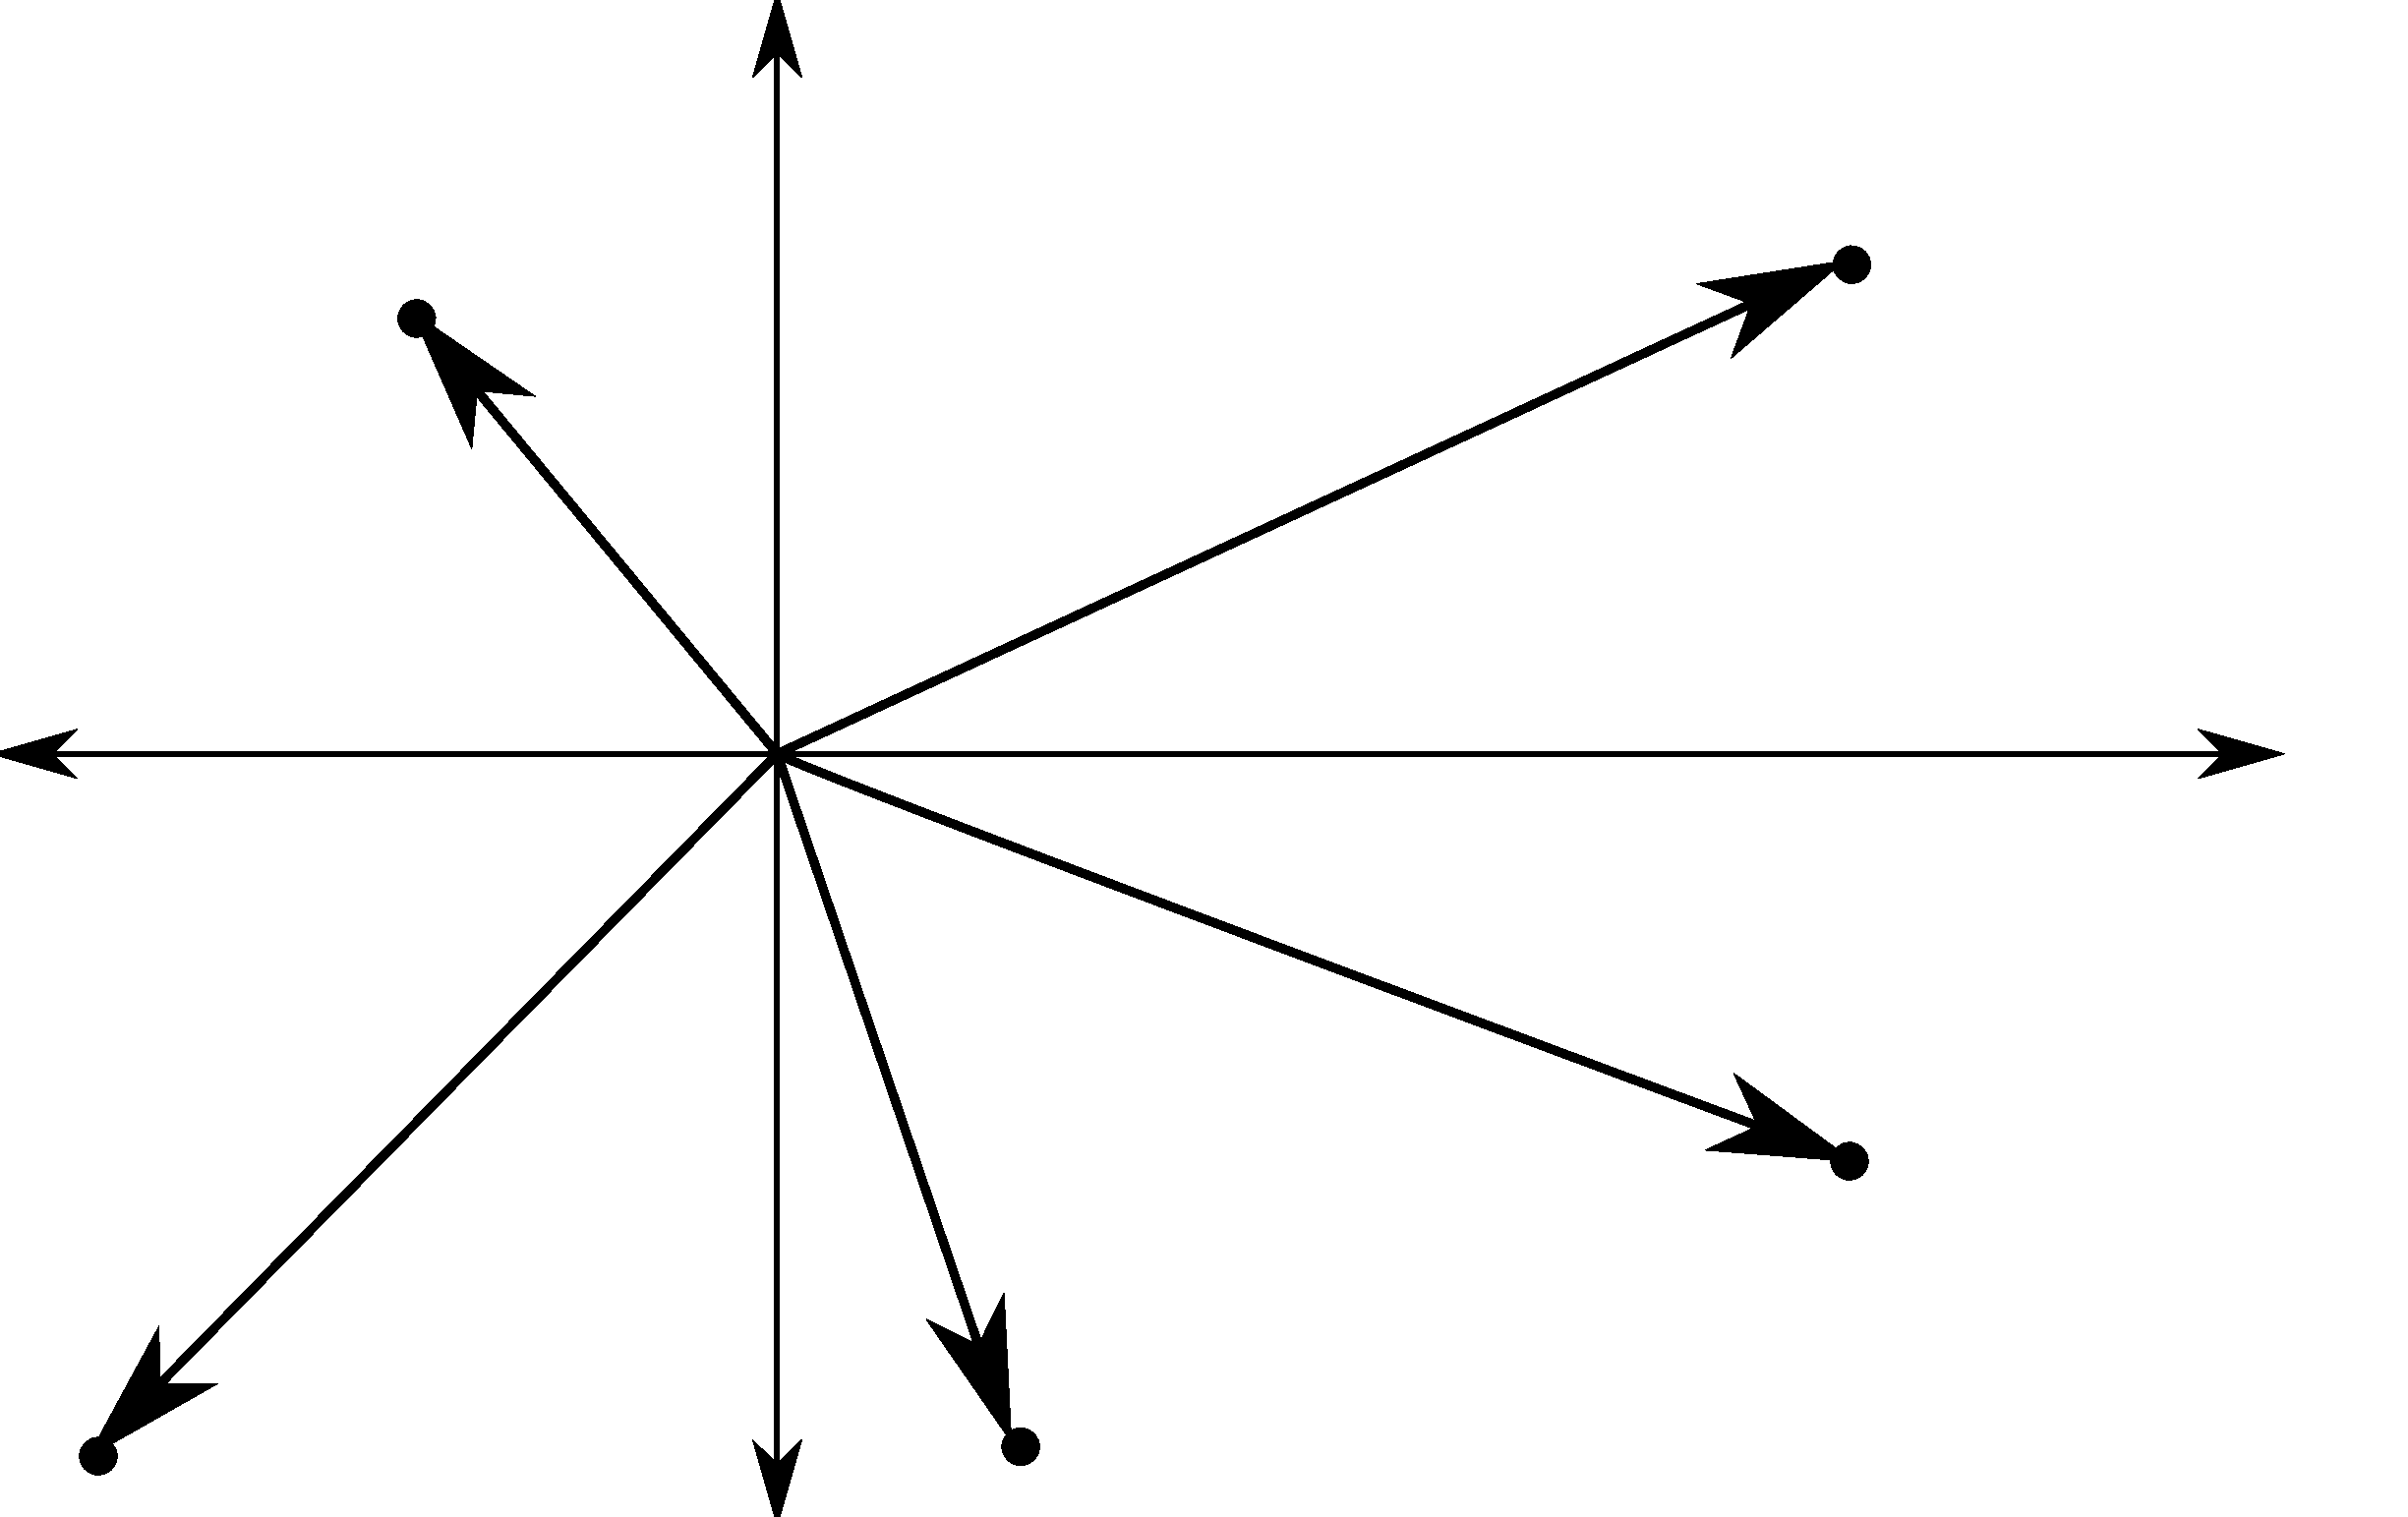
\includegraphics[width=3in]{argand2.pdf}
\end{center}
\end{frame}
\begin{frame}\frametitle{Addition of complex numbers}
 Addition of complex numbers is the same as the addition of geometric vectors in $\R^2$:

 If $z_1=x_1+iy_1$ and $z_2=x_2+iy_2$, then we define
\[
 z_1+z_2 = (x_1+iy_1)+(x_2+iy_2) = (x_1+x_2)+i(y_1+y_2)
\]

 {\bf Examples:} 

\end{frame}
\begin{frame}\frametitle{Properties of addition}
 Addition in $\C$ follows the same rules as addition in $\R$ (or $\R^2$):

 \begin{itemize}
  \item $z_1+z_2 = z_2+z_1$ for all $z_1,z_2\in\C$.
  \item $z_1+(z_2+z_3) = (z_1+z_2)+z_3$ for all $z_1,z_2,z_3\in \C$
  \item $0+z = z+0=z$ for all $z\in \C$, where $0 = 0 + i0$.
  \item Given $z=x+iy$, if we define $-z = -x-iy$, then $z+(-z)=-z+z=0$.
 \end{itemize}

\end{frame}
\begin{frame}\frametitle{Multiplication of complex numbers}
 A big difference between $\C$ and $\R^2$ (algebraically) is that we can \alert{multiply} complex numbers. Given $z=x+iy$ and $w=u+iv$, $zw$ is computed as a product of binomials, where we remember that $i^2=-1$:

 \[
  zw = (x+iy)(u+iv) = xu+ixv+iyu+i^2yv = (xu-yv)+i(xv+yu)
 \]

{\bf Examples:}

\end{frame}
\begin{frame}\frametitle{Multiplicative inverses}
 Given $z\in\C$ with $z\neq 0$, can we find a complex number $z^{-1}$ (or $1/z$) such that $zz^{-1}=1$?

 Say $z=x+iy$ and $w=u+iv$ satisfy $zw=1$. Then
\[
 zw = (xu-yv)+i(xv+yu) = 1 = 1+i0,
\]
which gives a system of equations in $u$ and $v$:
\[
 xu-yv = 1 \quad \text{ and } \quad xv+yu = 0.
\]
Solving gives $u=\dfrac{x}{x^2+y^2}$ and $v = \dfrac{-y}{x^2+y^2}$, which suggests:
\[
 \frac{1}{x+iy} = \frac{x}{x^2+y^2}-i\frac{y}{x^2+y^2}.
\]

\end{frame}
\begin{frame}\frametitle{Properties of complex multiplication}
 The results on the previous slide tell us that every nonzero complex number has a multiplicative inverse. One can check that the following properties all hold:
\begin{itemize}
 \item $z_1z_2=z_2z_1$ for all $z_1,z_2\in\C$.
 \item $z_1(z_2z_3)=(z_1z_2)z_3$ for all $z_1,z_2,z_3\in\C$.
 \item $1z = z1 = z$ for all $z\in\C$, where $1 = 1+i0$.
 \item For all $z\neq 0$, there exists $z^{-1}\in\C$ such that $zz^{-1}=z^{-1}z=1$
 \item $z_1(z_2+z_3) = z_1z_2+z_1z_3$ for all $z_1,z_2,z_3\in\C$
\end{itemize}

\end{frame}
\begin{frame}\frametitle{Elements of complex numbers}
For any $z=x+iy\in \C$, we define the following:
\begin{itemize}
\item The \alert{real part} of $z$, $\Re z = x$.
\item The \alert{imaginary part} of $z$, $\Im z = y$.
\item The \alert{complex conjugate} of $z$, $\overline{z} = x-iy$.
\item The \alert{modulus} of $z$, $\abs{z} = \sqrt{x^2+y^2}$.
\item The \alert{argument} of $z$, $\arg z = \theta$, where $\tan \theta = \frac{y}{z}$.
\end{itemize}
\begin{center}
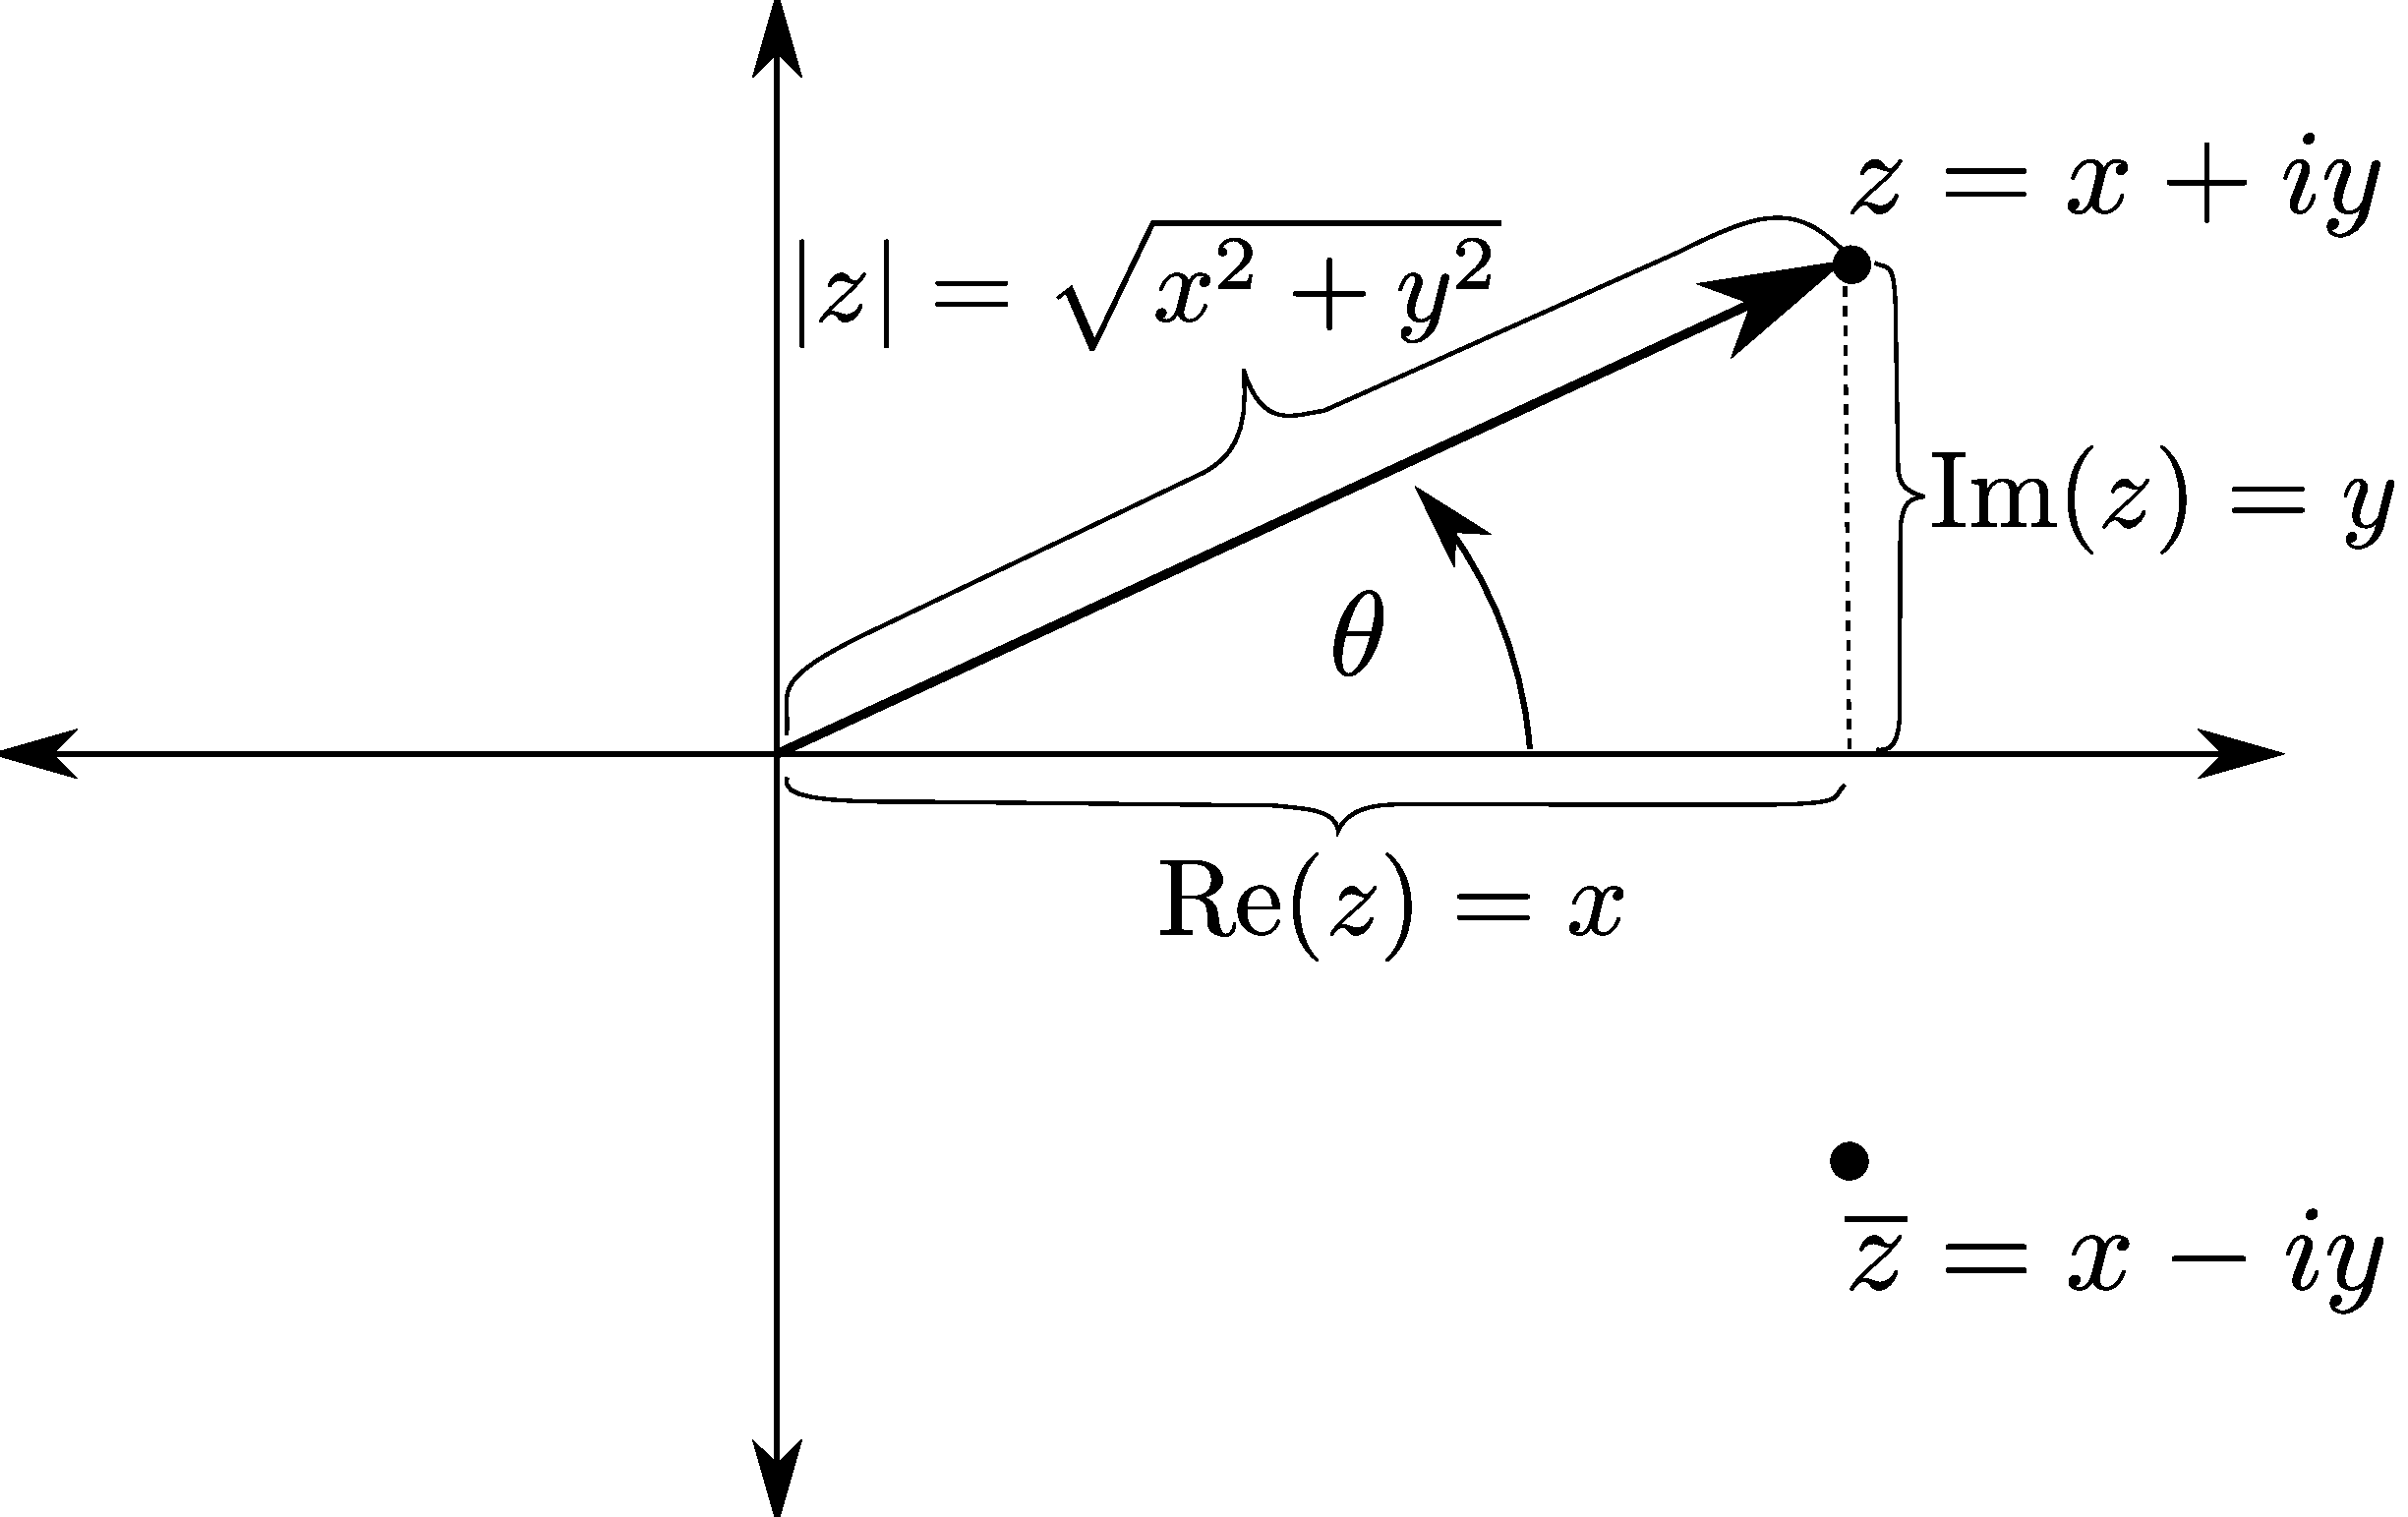
\includegraphics[width=3in]{argand.pdf}
\end{center}
\end{frame}
\begin{frame}
\frametitle{Division in $\C$}
We saw above that for every non-zero $z\in\C$, we can define $z^{-1} = \frac{x}{x^2+y^2}+i\frac{-y}{x^2+y^2}$ such that $zz^{-1}=1$.

In principle, this allows us to define division, but the result is hard to remember. Instead, we note the following:
\begin{theorem}
For all $z\in\C$, $z\overline{z} = \abs{z}^2$.
\end{theorem}
\begin{proof}
\vspace{0.5in}
\end{proof}
How does it help? $\abs{z}^2 = x^2+y^2$ is a \alert{real number}, and we know how to divide by real numbers.
\end{frame}
\begin{frame}
\frametitle{Examples}

\end{frame}
\begin{frame}
\frametitle{A matrix model for $\C$}
If you find the idea of defining a number $i$ such that $i^2=-1$, consider the following:

Let $V$ denote the set of all $2\times 2$ matrices. Let $\mathbf{1}=\begin{bmatrix}1&0\\0&1\end{bmatrix}\in V$, and recall that this matrix satisfies $A\mathbf{1}=\mathbf{1}A=A$ for all $A\in V$.

Now, let $U\subseteq V$ denote the subset
\[
U = \left\{\left.\begin{bmatrix}x&y\\-y&x\end{bmatrix}\,\right|\, x,y\in\R\right\}.
\]
Notice that if $A\in U$, then $A = x\mathbf{1}+y\mathbf{i}$, where $\mathbf{i}=\begin{bmatrix}0&1\\-1&0\end{bmatrix}$.
\end{frame}
\begin{frame}
\frametitle{The polar form of a complex number}
Given $z=x+iy$, we have $\abs{z}=\sqrt{x^2+y^2}$, and if $\theta = \arg z = \tan^{-1}(y/x)$, then basic trigonometry tells us
\begin{align*}
 x & = \abs{z}\cos\theta\\
 y & = \abs{z}\sin\theta
\end{align*}
Thus, if we let $r=\abs{z}$, we can write any $z\in \C$ in \alert{polar form} as
\[
z = r\cos\theta +ir\sin\theta.
\]

\alert{Note:} For the above to be well-defined, we have to define a ``branch'' of the argument: there are infinitely many values of $\theta$ that work. We'll require $\theta\in (-\pi,\pi]$. (Some texts take $\theta \in [0,2\pi)$.)
\end{frame}
\begin{frame}\frametitle{Euler's Formula}
\alert{Euler's identity} is one of the most remarkable formulas in mathematics: we define the complex exponential $e^{i\theta}$ by
\[
e^{i\theta} = \cos\theta+i\sin\theta.
\]
This is usually taken as a definition, although there are several motivations for it. In particular, using the angle addition trigonometric identities, we find that
\begin{align*}
e^{i(\alpha+\beta)} &= \cos(\alpha+\beta) + i\sin(\alpha+\beta)\\
& = \cos\alpha\cos\beta - \sin\alpha\sin\beta + i(\sin\alpha\cos\beta+\cos\alpha\sin\beta)\\
& = (\cos\alpha + i\sin\alpha)(\cos\beta+i\sin\beta)\\
& = e^{i\alpha}e^{i\beta}
\end{align*}
Another famous result, called \alert{de Moivre's theorem}, asserts that for all natural numbers $n$,
\[
(e^{i\theta})^n = (\cos\theta+i\sin \theta)^n = \cos n\theta + i\sin n\theta = e^{in\theta}.
\]

\end{frame}
\begin{frame}
\frametitle{Examples}
\begin{enumerate}
\item Find the values of $e^{i\pi/4}, e^{i\pi/2}, e^{i\pi}$ and $e^{i2\pi/3}$.

\vspace{1.5in}

\item Show that $e^{i\theta} = e^{i(\theta+2\pi k)}$ for all integers $k$.
\end{enumerate}
\end{frame}
\begin{frame}
\frametitle{Example}

Establish trigonometric identities for $\cos 3\theta$ and $\sin 3\theta$.

\end{frame}
\begin{frame}
\frametitle{Polar form, again}
If we introduce polar coordinates $r = \sqrt{x^2+y^2}$ and $\theta\in (-\pi,\pi]$ such that $\tan\theta = y/x$, we can write
\[
z = \abs{z}\cos\theta+i\abs{z}\sin\theta = re^{i\theta},
\]
with the help of Euler's theorem. This form of a complex number can be very convenient. For one thing, we will see that it makes finding roots of complex numbers much easier. For another, it gives us a geometric interpretation of complex multiplication.
\end{frame}
\begin{frame}
\frametitle{Example}

Compute $(1+i)^5$.
\end{frame}
\begin{frame}
\frametitle{Roots of complex numbers}

Polar coordinates make it easy to solve equations of the form $z^n=w$.

Given $w=u+iv$, re-write in polar form: $w = ae^{i\phi}$. If $z=re^{i\theta}$, then $z^n=w$ becomes
\[
r^ne^{in\theta} = ae^{i\phi} = ae^{i(\phi+2\pi k)}, \, k=0,1,2,\ldots.
\]
Solutions: $r = a^{1/n}$, and $\theta = \dfrac{\phi}{n}+\dfrac{2k}{n}\pi$, $k=0,1,2,\ldots$
\end{frame}
\begin{frame}
\frametitle{Examples}

Solve the following equations: $z^6=1$, and $z^4=16i$.
\end{frame}
\begin{frame}
\frametitle{The Fundamental Theorem of Algebra}
Complex numbers don't just allow us to solve quadratic or cubic equations involving real numbers. In fact, we have the following remarkable theorem:
\begin{theorem}
Let $p(z) = a_0+a_1z+a_2z^2+\cdots + a_nz^n$ be any polynomial with complex coefficients $a_0,a_1,\ldots, a_n\in\C$, $n\geq 1$. Then $p$ has a root.
\end{theorem}
Consequence: every polynomial -- even with complex coefficients -- can be \alert{completely factored} over $\C$.
\end{frame}
\end{document}